%!TeX root=../tese.tex
%("dica" para o editor de texto: este arquivo é parte de um documento maior)
% para saber mais: https://tex.stackexchange.com/q/78101/183146

%% ------------------------------------------------------------------------- %%
\chapter{\textit{Generator Demo}}
\label{ap:generator demo}

A cena \textit{Generator Demo} consiste em uma fase com apenas um inimigo imortal, o personagem e um \textit{menu} na lateral esquerda da tela. O menu permite o controle dos geradores do inimigo, permitindo adicionar geradores, selecionar um gerador criado e alterar qualquer parâmetro deste para testes. As alterações são refletidas no gerador selecionado em tempo real, facilitando a visualização de resultados de diferentes combinações de valores e auxiliando na escrita de fases e inimigos mais diversos.

\begin{figure}
    \centering

    \begin{subfigure}{1\textwidth}
        \centering
        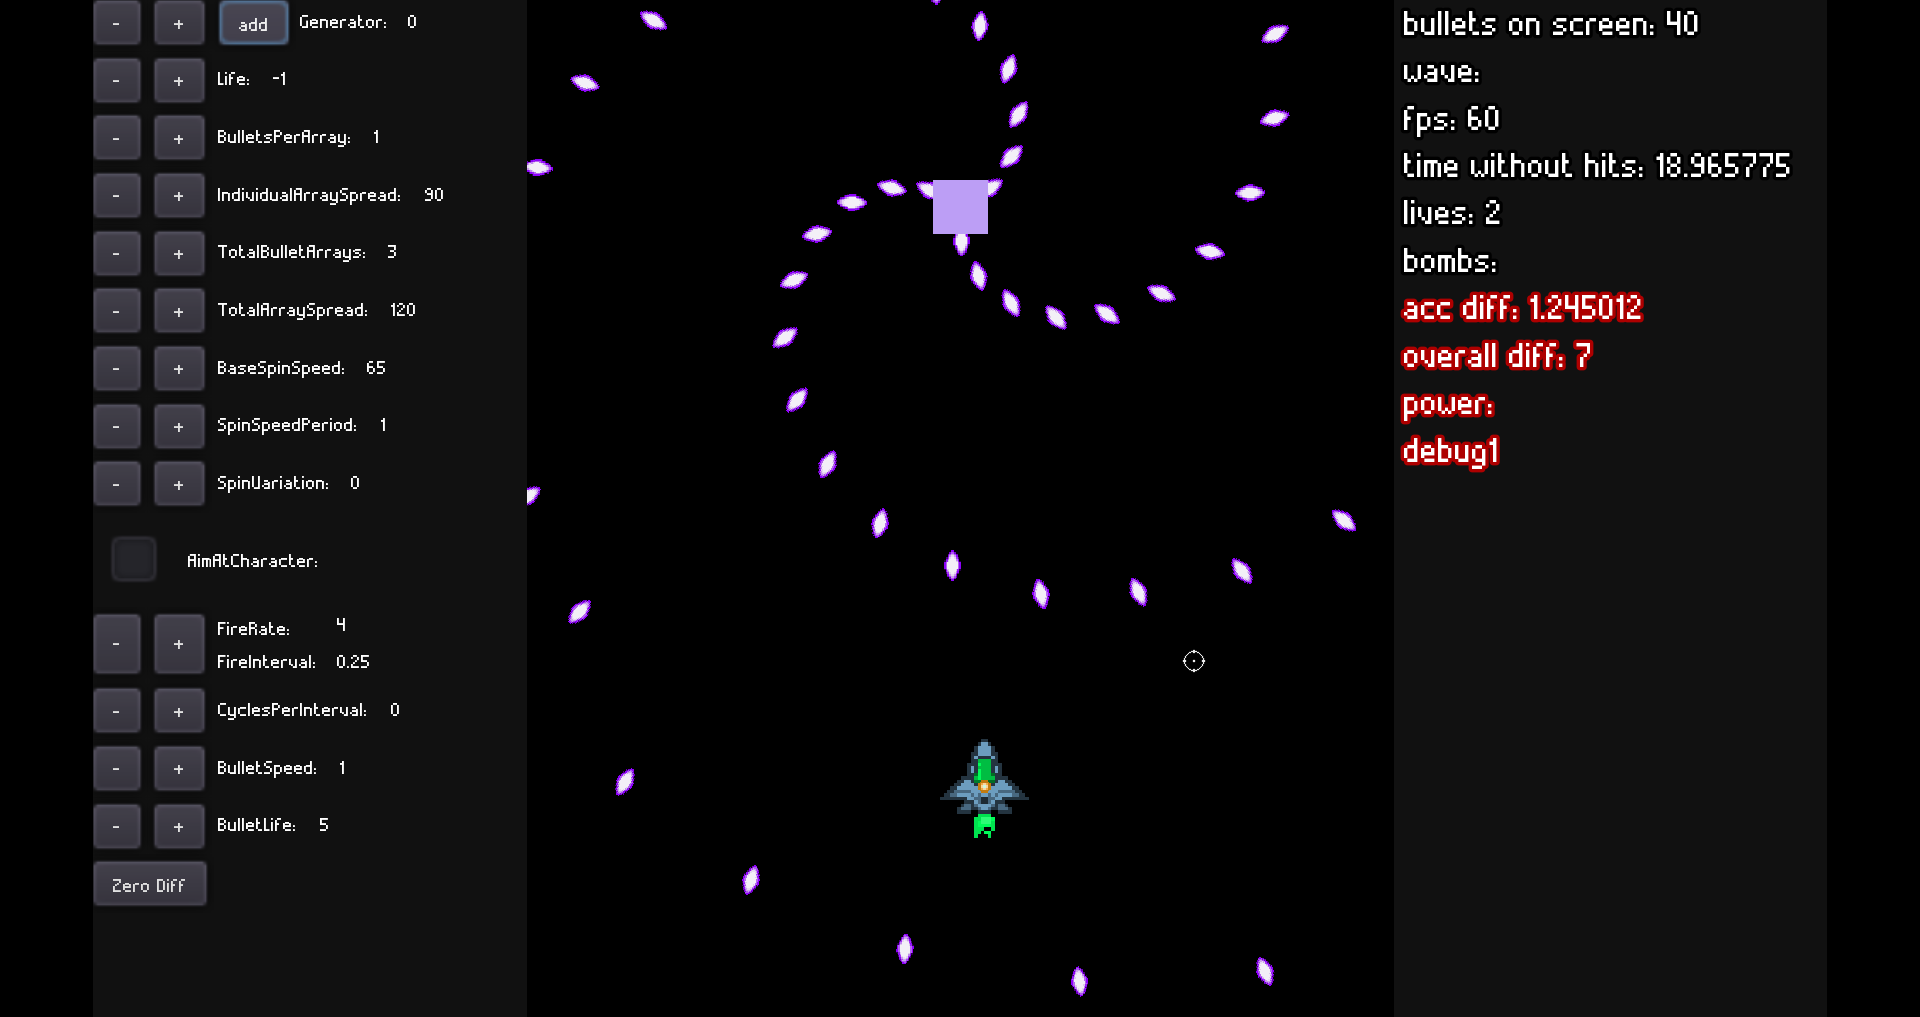
\includegraphics[width=1\textwidth]{generatorDemo}
    \end{subfigure}

    \caption{Cena de demonstração de gerador de projéteis.\label{generatorDemo}}
\end{figure}
